Più in dettaglio, abbiamo suddiviso ulteriormente il model in:
\begin{itemize}
	\item POSManager: parte dell'applicazione che si occupa dell'uso del software di apprendimento automatico;
	\item Data: l'insieme delle classi di business che permettono di svolgere le operazione di calcolo sui dati estratti dal database;
	\item Firebase: insieme di classi usate per l'utilizzo del database fornito da Firebase;
	\item Database: insieme di classi che utilizzano quelle definite dal pacchetto Firebase e che disaccoppiano l'applicazione dall'implementazione del database;
	\item Client: il cui scopo è esporre le funzionalità del model.
\end{itemize}
\begin{figure}[h]
	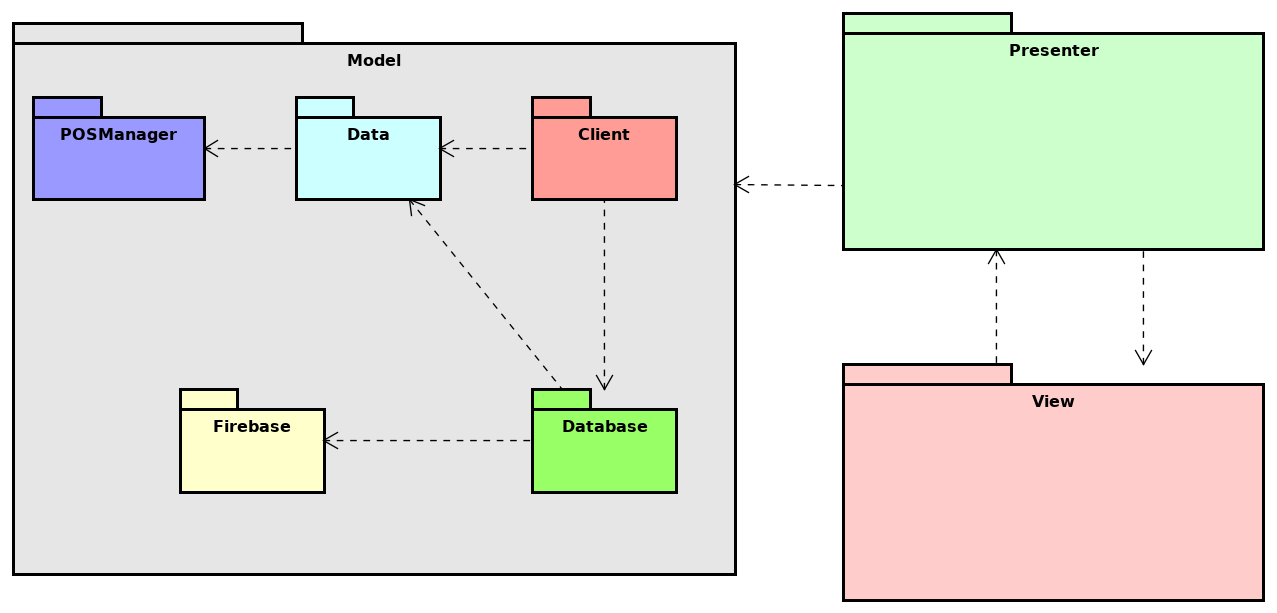
\includegraphics[scale=0.5]{images/package.png}
	\caption{Diagramma dei package}
\end{figure}